\begin{figure}
	\begin{minipage}[b]{.5\linewidth}
		\centering
		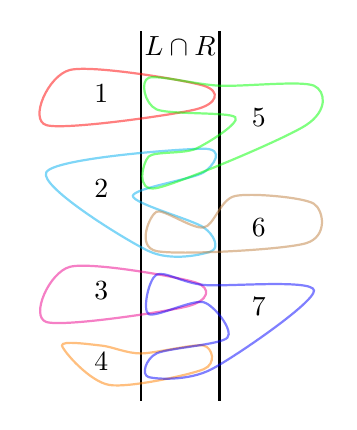
\begin{tikzpicture}		
			\draw[thick] (-.5,-.7) -- (-.5,4);		
			\draw[thick] (.5,-.7) -- (.5,4);				
			\node at (0,3.8){$ L \cap R $};
			\draw [red, thick, opacity=.5] plot [smooth cycle] coordinates {(-1.4,3.5) (.3,3.3) (.2,3) (-1.7, 2.8)}; \node at (-1,3.2){1}; %1
			\draw [cyan, thick, opacity=.5] plot [smooth cycle] coordinates {(-1.7,2.2) (.3,2.5) (.3,2.2) (-.6,1.9) (.3,1.5) (.4,1.2) (-.4,1.2)}; \node at (-1,2){2};%2
			\draw [magenta, thick, opacity=.5] plot [smooth cycle] coordinates {(-1.4,1) (.2,0.8) (.1,.5) (-1.7,.3)}; \node at (-1,.7){3};%3
			\draw [orange, thick, opacity=.5] plot [smooth cycle] coordinates {(-1.5,0) (-1,0) (-.5,-.1) (.3,0) (.3,-.3) (-.9,-.5)}; \node at (-1,-.2){4};%4
			\draw [green, thick, opacity=.5] plot [smooth cycle] coordinates {(-.4,3.4) (.5,3.3) (1.7,3.3) (1.6,2.8) (-.3,2) (-.4,2.4) (.2,2.5) (.7,2.9) (-.3,3)}; \node at (1,2.9){5};%5
			\draw [brown, thick, opacity=.5] plot [smooth cycle] coordinates {(1.7,1.8) (1.6,1.3) (-.3,1.2) (-.3,1.7) (.3,1.5) (.7,1.9)}; \node at (1,1.5){6};%6
			\draw [blue, thick, opacity=.5] plot [smooth cycle] coordinates {(1.7,.7) (.3,.77) (-.3,.9) (-.4,.4) (.3,.55) (.6,.1) (-.3,-.1) (-.4,-.4) (.4,-.3)}; \node at (1,.5){7};%7
		\end{tikzpicture}
		\subcaption{przykładowe grupy}\label{qscan:cid-graph-groups}
	\end{minipage}%
	\begin{minipage}[b]{.5\linewidth}
		\centering
		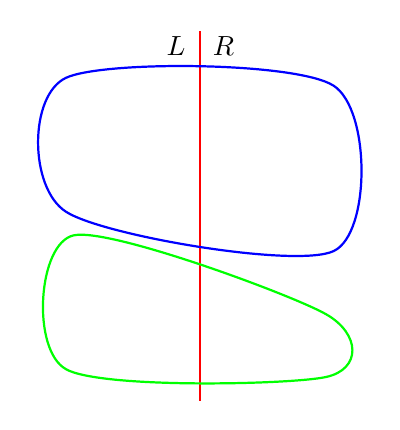
\begin{tikzpicture}
			\GraphInit[vstyle=Normal]
			\Vertex[x=0,y=3]{1}
			\Vertex[x=0,y=2]{2}
			\Vertex[x=0,y=1]{3}
			\Vertex[x=0,y=0]{4}
			\Vertex[x=3,y=3]{5}
			\Vertex[x=3,y=1.5]{6}
			\Vertex[x=3,y=0]{7}
			\Edges(1,5,2,6)
			\Edges(4,7,3)
			
			\draw[red,thick] (1.5,-.7) -- (1.5,4);			
			\node at (1.2,3.8){$ L $};
			\node at (1.8,3.8){$ R $};	
			\draw [blue, thick] plot [smooth cycle] coordinates {(-.2,3.4) (-.2,1.7) (3.2,1.2) (3.2,3.3)};
			\draw [green, thick] plot [smooth cycle] coordinates {(-.1,1.4) (-.2,-.3) (3.1,-.4) (3.1,.4)};
		\end{tikzpicture}
		\subcaption{graf zależności i uspójnione grupy}\label{qscan:cid-graph-graph}
	\end{minipage}
	\caption{Graf zależności \subref{qscan:cid-graph-graph} pomiędzy etykietami grup w podzbiorach $ L $ oraz $ R $ dla przykładowego rozkładu grup \subref{qscan:cid-graph-groups}. }\label{qscan:cid-graph}
\end{figure}